\documentclass[aspectratio=169, lecture, amberg]{OTHAWbeamer}
\let\Tiny=\tiny  
\usepackage{ngerman}
\usepackage{amssymb}
\usepackage[utf8]{inputenc}
\usepackage{etex}
\usepackage{biblatex}
\addbibresource{references.bib}

\title[Forschungsseminar]{One-Step Image Translation with Text-to-Image Models}
\subtitle{Forschungsseminar}
\author[Schmidt]{Fabian Schmidt}
\place{OTH Amberg-Weiden}
\date{\today}


\email{f.schmidt3@oth-aw.de}

\begin{document}
\maketitle

% ---------- Begin Präsentation ----------
\frame{
\frametitle{Tabel of Contents}
\begin{enumerate}
    \item Introduction
    \item Related Work
    \item Terminology
    \item Method
    \item Experiments
    \item Discussion and Limitations
    \item Live Demo
\end{enumerate}
\tableofcontents
}
% ---------- Begin Section Introduction ----------
% ---------- Problems with Diffusion Models ----------
\begin{frame}
\frametitle{Introduction}
\framesubtitle{Problems with Diffusion Models}

\begin{columns}
    \column{0.5\textwidth}
    \centering
    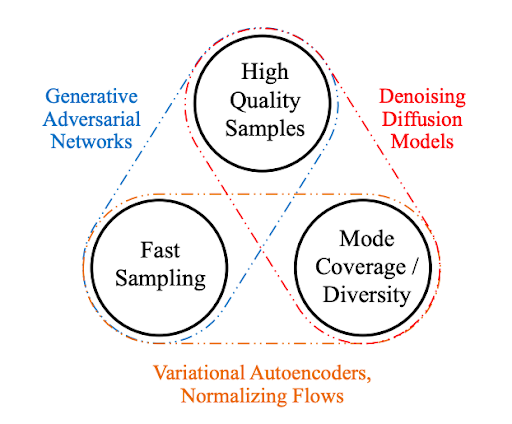
\includegraphics[width=0.9\textwidth]{images/GANs_Diffusion_Autoencoders.png}

    \column{0.5\textwidth}
    \centering
    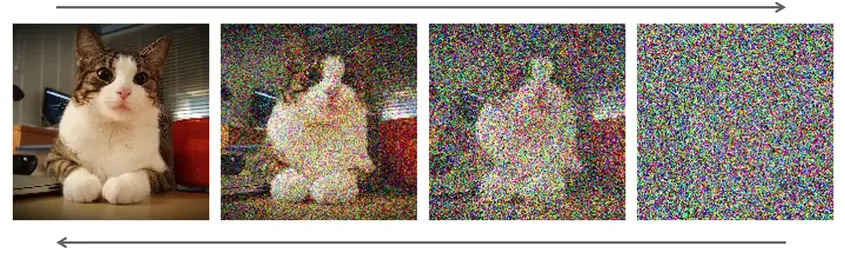
\includegraphics[width=\textwidth]{images/Generation-with-Diffusion-Models-ezgif.com-webp-to-jpg-converter.jpg}
  \end{columns}  
  \tiny{\footnotemark \url{https://developer.nvidia.com/blog/improving-diffusion-models-as-an-alternative-to-gans-part-1/}}
  \tiny{\footnotemark \url{https://miro.medium.com/v2/resize:fit:720/format:webp/1*RDPhd2dvmHE4UrAP-QHb9w.png}}
\end{frame}

% ---------- Proposed solutions ----------
\begin{frame}
\frametitle{Introduction}
\framesubtitle{Proposed solutions}
\begin{itemize}
    \item One-step image-to-image translation method for paired and unpaired settings
    \item Reduce number of inference steps to 1
    \item Trainable without image pairs
    \item Adapt pre-trained text-conditional one-step diffusion model to new domains via adversarial learning
\end{itemize}
\end{frame}

% ---------- Begin Section Related Work ----------
% ---------- Image-to-Image translation ----------
\begin{frame}
\frametitle{Related Work}
\framesubtitle{Image-to-Image translation}
Paired Image Translation
\begin{itemize}
    \item e.g. GLIGEN \cite{li2023gligen}, T2I-Adapter \cite{mou2023t2i}, ControlNet \cite{zhang2023adding}
    \item requires large number of training pairs
    \item slow inference
\end{itemize}
Unpaired Image Translation
\begin{itemize}
    \item GAN- or diffusion-based methods \cite{cyclediffusion} \cite{su2022dual} \cite{sasaki2021unitddpm}
    \item require training from scratch on new domains   
\end{itemize}
\end{frame}

% ---------- Text-to-Image models ----------
\begin{frame}
\frametitle{Related Work}
\framesubtitle{Text-to-Image models}

\end{frame}

% ---------- One-step generative models ----------
\begin{frame}
\frametitle{Related Work}
\framesubtitle{One-step generative models}

\end{frame}

% ---------- Begin Section Terminology ----------
% ---------- Generative Adversarial Networks(GAN) ----------
\begin{frame}
\frametitle{Terminology}
\framesubtitle{Generative Adversarial Networks(GAN)}
\begin{figure}
    \centering
    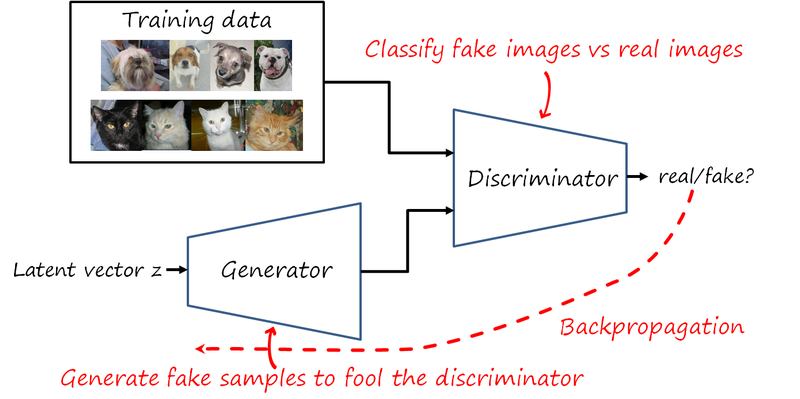
\includegraphics[width=0.65\linewidth]{images/blog_gan.png}
    \caption{GAN training process}
\end{figure}
\tiny{\footnotemark \url{http://www.lherranz.org/2018/08/07/imagetranslation/}}
\end{frame}
\note{}

% ---------- Generative Adversarial Networks(GAN) ----------
\begin{frame}
    \frametitle{Terminology}
    \framesubtitle{Generative Adversarial Networks(GAN)}
    \begin{block}{Generator loss}
        \begin{equation}
            \min_G \mathcal{L}_G = \mathbb{E}_{z \sim p_z(z)} [\log(1 - D(G(z)))]
        \end{equation}
    \end{block}
    \begin{block}{Discriminator loss}
        \begin{equation}
            \max_D \mathcal{L}_D = \mathbb{E}_{x \sim p_{\text{data}}(x)} [\log D(x)] + \mathbb{E}_{z \sim p_z(z)} [\log(1 - D(G(z)))]
        \end{equation}
    \end{block}
    \tiny\footnotemark \url{Goodfellow, I., Pouget-Abadie, J., Mirza, M., Xu, B., Warde-Farley, D., Ozair,
    S., Courville, A., Bengio, Y.: Generative adversarial nets. In: Neural Information
    Processing Systems (NeurIPS) (2014)}
\end{frame}

% ---------- CycleGAN ----------
\begin{frame}
\frametitle{Terminology}
\framesubtitle{CycleGAN}
\begin{figure}
    \centering
    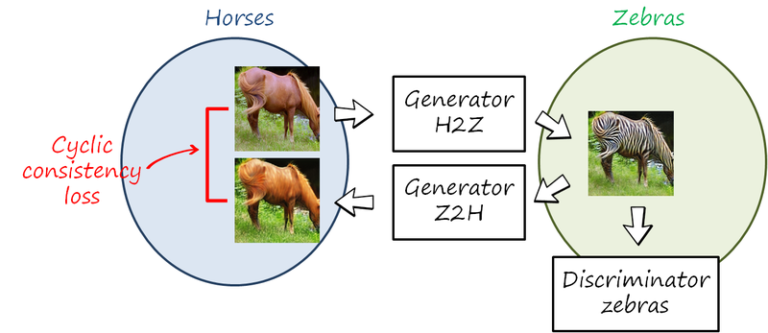
\includegraphics[width=0.78\linewidth]{images/blog_cyclegan_h2z2h-768x333.png}
    \caption{CycleGAN Architecture}
\end{figure}
\tiny{\footnotemark \url{http://www.lherranz.org/2018/08/07/imagetranslation/}}
\end{frame}

% ---------- CycleGAN ----------
\begin{frame}
    \frametitle{Terminology}
    \framesubtitle{CycleGAN}
    \begin{block}{Adversarial loss for G}
        \begin{equation}
            \mathcal{L}_{\text{GAN}}(G, D_Y, X, Y) = \mathbb{E}_{y \sim p_{\text{data}}(y)} [\log D_Y(y)] + \mathbb{E}_{x \sim p_{\text{data}}(x)} [\log(1 - D_Y(G(x)))]
        \end{equation}
    \end{block}

    \begin{block}{Adversarial loss for F}
        \begin{equation}
            \mathcal{L}_{\text{GAN}}(F, D_X, Y, X) = \mathbb{E}_{x \sim p_{\text{data}}(x)} [\log D_X(x)] + \mathbb{E}_{y \sim p_{\text{data}}(y)} [\log(1 - D_X(F(y)))]
        \end{equation}
    \end{block}

    \begin{block}{Cycle consistency loss}
        \begin{equation}
        \mathcal{L}_{\text{cycle}}(G, F) = \mathbb{E}_{x \sim p_{\text{data}}(x)} [\lVert F(G(x)) - x \rVert_1] + \mathbb{E}_{y \sim p_{\text{data}}(y)} [\lVert G(F(y)) - y \rVert_1]
        \end{equation}
    \end{block}
\end{frame}

% ---------- CycleGAN ----------
\begin{frame}
    \frametitle{Terminology}
    \framesubtitle{CycleGAN}
    \begin{block}{Identity loss}
        \begin{align}
            \mathcal{L}_{\text{identity}}(G, F, X, Y) & = \mathbb{E}_{y \sim p_{\text{data}}(y)} [\lVert G(y) - y \rVert_1] \\
            \mathcal{L}_{\text{identity}}(F, G, Y, X) & = \mathbb{E}_{x \sim p_{\text{data}}(x)} [\lVert F(x) - x \rVert_1]
        \end{align}
    \end{block}

    \begin{block}{Cycle loss}
        \begin{equation}
            \begin{split}
                &\mathcal{L}(G, F, D_X, D_Y) = \mathcal{L}_{\text{GAN}}(G, D_Y, X, Y) + \mathcal{L}_{\text{GAN}}(F, D_X, Y, X) + \\
                &\lambda \mathcal{L}_{\text{cycle}}(G, F) + \lambda_{\text{id}} \left( \mathcal{L}_{\text{identity}}(G, F, X, Y) + \mathcal{L}_{\text{identity}}(F, G, Y, X) \right)
            \end{split}    
        \end{equation}
    \end{block}
\end{frame}
\note{stuff here}

% ---------- Paired vs unpaired data ----------
\begin{frame}
\frametitle{Terminology}
\framesubtitle{Paired vs unpaired data}
\begin{columns}
    \column{0.5\textwidth}
    \centering    
    \begin{figure}
        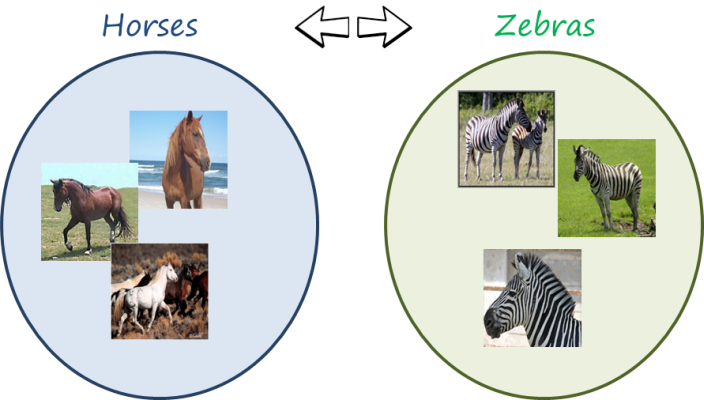
\includegraphics[width=0.75\textwidth]{images/blog_unpairedimagetranslation2.png}
        \caption{Unpaired Data}
    \end{figure}

    \column{0.5\textwidth}    
    \centering    
    \begin{figure}        
        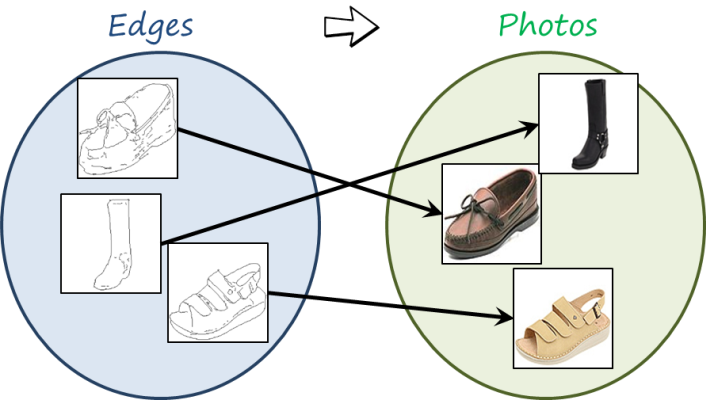
\includegraphics[width=0.75\textwidth]{images/blog_pairedimagetranslation.png}
        \caption{Paired Data}
    \end{figure}
  \end{columns}
\end{frame}

% ---------- UNet and Skip Connections ----------
\begin{frame}
\frametitle{Terminology}
\framesubtitle{UNet and Skip Connections}
\begin{figure}
    \centering
    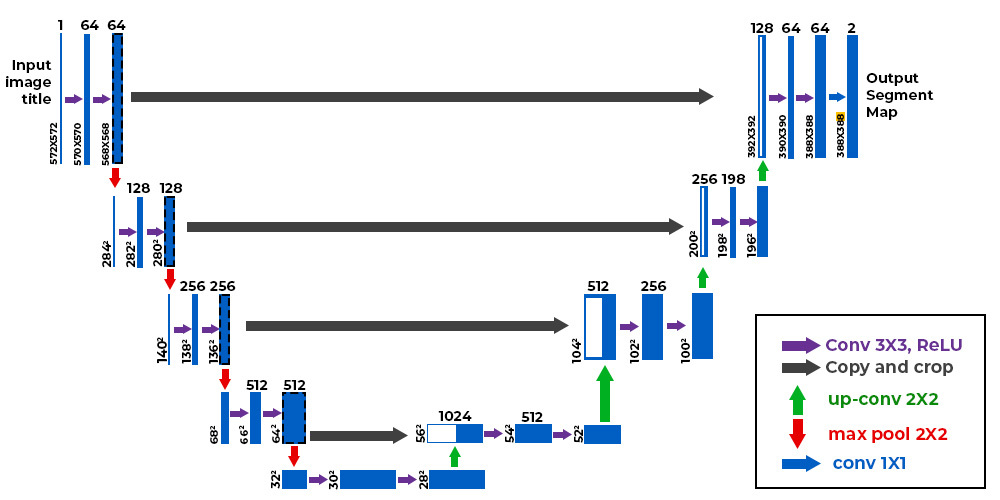
\includegraphics[width=0.6\linewidth]{images/Group14.jpg}
    \caption{Architecture}
\end{figure}
\end{frame}

% ---------- LoRA Weights ----------
\begin{frame}
\frametitle{Terminology}
\framesubtitle{LoRA Weights}
\begin{figure}
    \centering
    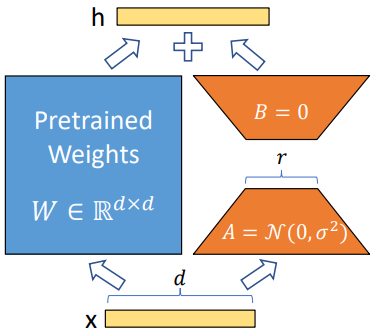
\includegraphics[width=0.4\linewidth]{images/Bildschirmfoto vom 2024-04-15 10-21-59.png}
    \caption{\textbf{Lo}w \textbf{R}ank \textbf{A}daption}
\end{figure}
\end{frame}

% ---------- Stabel Diffusion ----------
\begin{frame}
\frametitle{Terminology}
\framesubtitle{Stable Diffusion}

\end{frame}

% ---------- Method ----------
% ---------- Goal ----------
\begin{frame}
\frametitle{Method}
\framesubtitle{Goal}
?
\end{frame}

% ---------- Adding Conditioning Input ----------
\begin{frame}
\frametitle{Method}
\framesubtitle{Adding Conditioning Input}
\begin{figure}
    \centering
    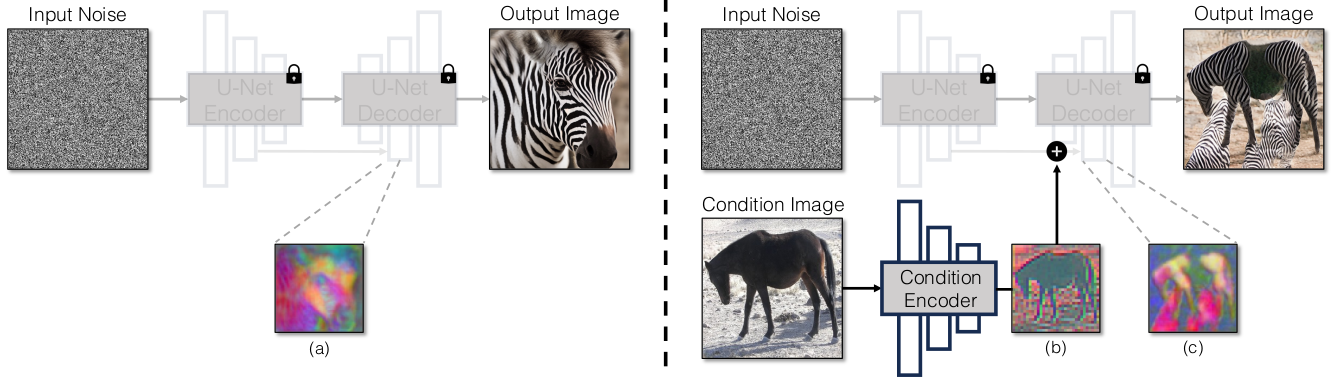
\includegraphics[width=1\linewidth]{images/Bildschirmfoto vom 2024-04-14 10-57-39.png}
    \caption{Enter Caption}
\end{figure}
\end{frame}

% ---------- Preserving Input Details ----------
\begin{frame}
\frametitle{Method}
\framesubtitle{Preserving Input Details}
\begin{figure}
    \centering
    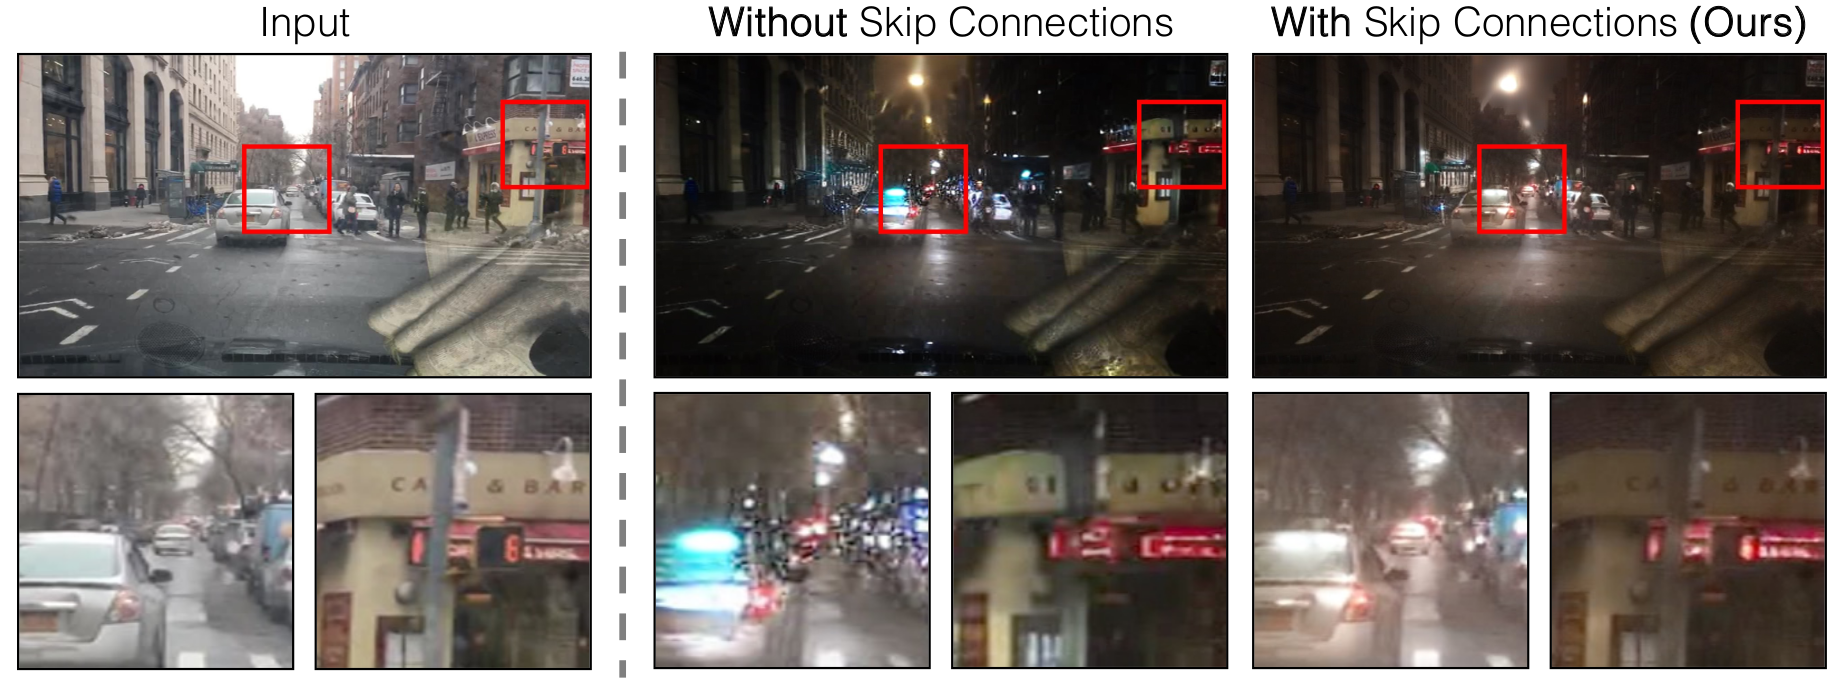
\includegraphics[width=1\linewidth]{images/Bildschirmfoto vom 2024-04-14 11-06-40.png}
    \caption{Skip Connections help retain details}
\end{figure}
\end{frame}

% ---------- Preserving Input Details ----------
\begin{frame}
\frametitle{Method}
\framesubtitle{Preserving Input Details}
\begin{figure}
    \centering
    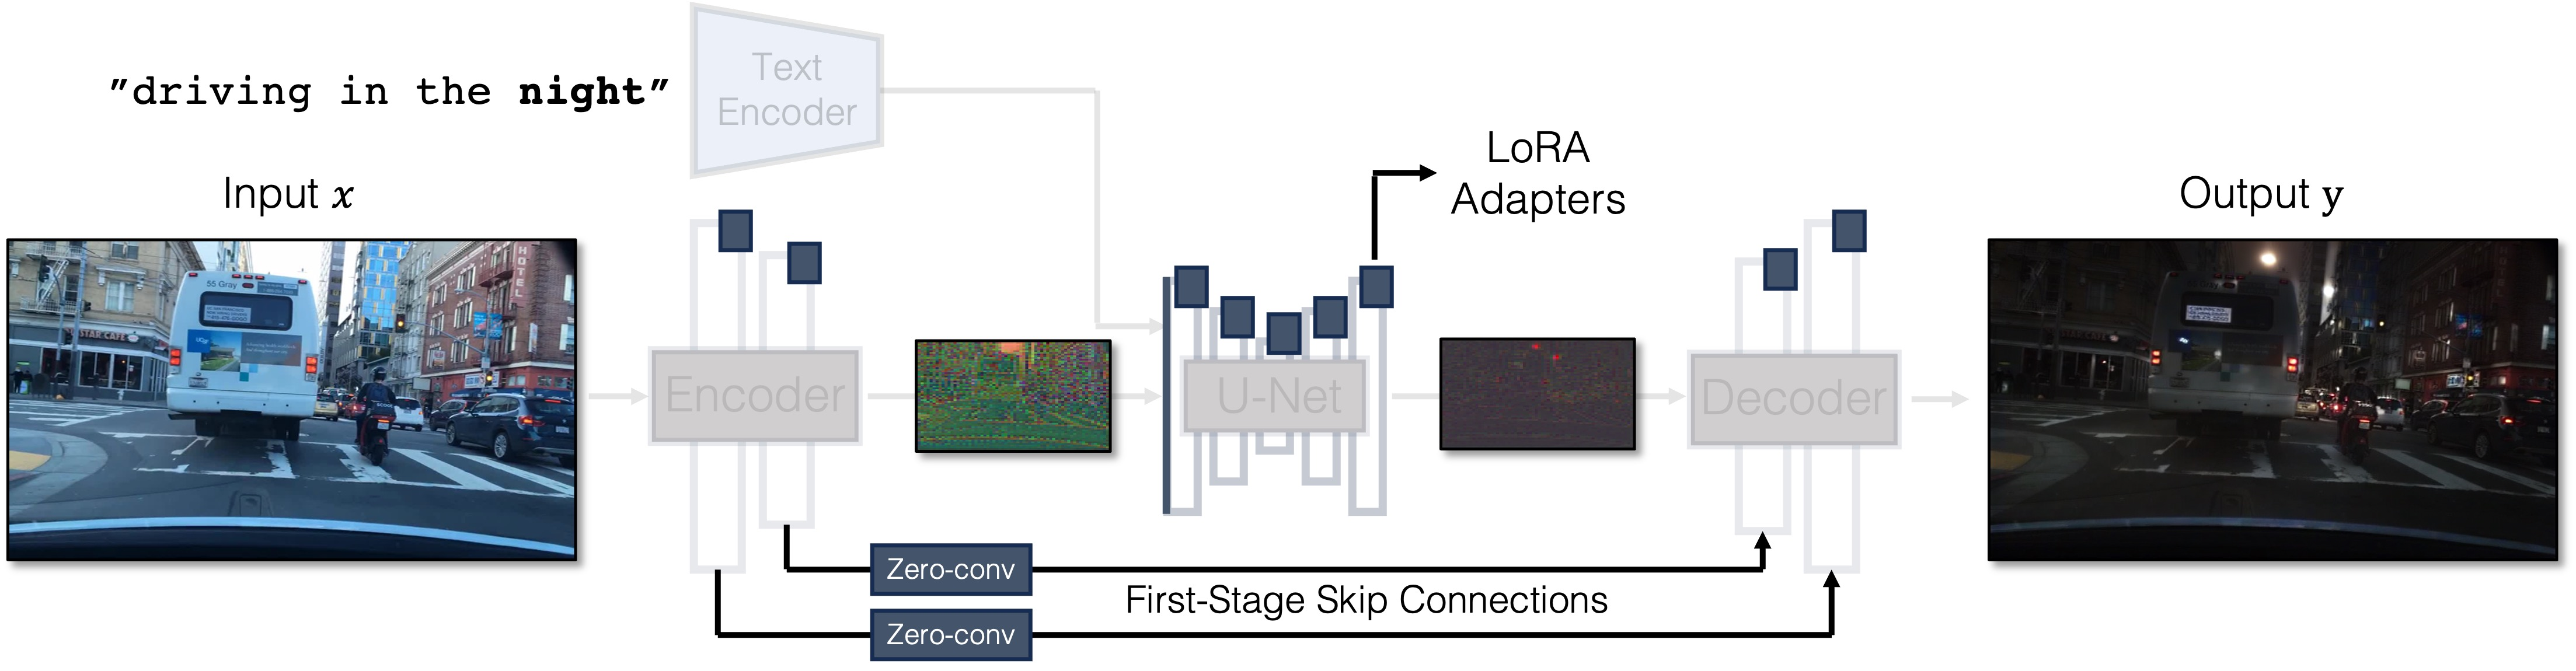
\includegraphics[width=1\linewidth]{images/method.jpg}
    \caption{Model Architecture}
\end{figure}
\end{frame}

% ---------- Unpaired Training ----------
\begin{frame}
\frametitle{Method}
\framesubtitle{Unpaired Training}

\end{frame}

% ---------- Extensions ----------
\begin{frame}
\frametitle{Method}
\framesubtitle{Extensions}

\end{frame}

% ---------- Begin Sections Experiments ----------
% ---------- Experiments ----------
\begin{frame}
\frametitle{Experiments}

\end{frame}

% ---------- Comparison to Unpaired Methods ----------
\begin{frame}
\frametitle{Experiments}
\framesubtitle{Comparison to Unpaired Methods}

\end{frame}

% ---------- Ablation Study ----------
\begin{frame}
\frametitle{Experiments}
\framesubtitle{Ablation Study}

\end{frame}

% ---------- Extensions ----------
\begin{frame}
\frametitle{Experiments}
\framesubtitle{Extensions}

\end{frame}

% ---------- Begin Section Discussion ----------
% ---------- Discussion ----------
\begin{frame}
\frametitle{Discussion and Limitations}
\framesubtitle{Discussion}
\begin{itemize}
    \item one-step pre-trained models can serve as a backbone model for many image synthesis tasks
    \item Adapting the models can be achieved through GAN objectives without multi-step diffusion training
    \item model training requires a small number of additional trainable parameters
\end{itemize}
\end{frame}

% ---------- Limitations ----------
\begin{frame}
\frametitle{Discussion and Limitations}
\framesubtitle{Limitations}
\begin{itemize}
    \item cannot specify strength of guidance as SD-Turbo does not use classifier-free guidance
    \item does not support negative prompt
    \item training is memory intensive
\end{itemize}

\end{frame}

% ---------- End ----------
\begin{frame}
\frametitle{The End}
\begin{center}
\scalebox{2}{Questions?}
\end{center}
\end{frame}
\end{document}

